\documentclass{article}
\usepackage[utf8]{inputenc}
\usepackage{tabularx}
\usepackage[letterpaper,total={5.5in,9in}, top=1.0in, inner=1.5in, outer=1.0in,bottom=1.0in,,headheight=0pt,headsep=0pt,centering]{geometry}
\title{BIOS14 - Final Exam}
\author{Pham Xuan Huy Nguyen}
\date{January 2023}
\usepackage{listings}
\usepackage{graphicx}
\begin{document}

\maketitle

\section{Effect of living conditions on the width of the lower bract on two species of \textit{Dalechampia}}
\textbf{Background}\\

Flower is one of the most important part in flowering plants and the condition of living can affect on floral parts. The bract's function in flower is not only provide protection but also attract pollinator. In this research, we will investigate the effect of different living treatments (dry/wet) on two species of \textit{Dalechampia} plant on the lower bract width (LWD).\\
\\
\textbf{Methods and Results}\\

The data was visualised by a mean plot with errors bar for each species, different colors indicate different treatments. From Figure \ref{fig1}, the LBW is higher in specie L and in treatment with wet. The LBW mean is different between dry and wet treatment across two species and the difference in LBW mean seems bigger in wet treatment.\\
\begin{figure}[h!]
\begin{center}
  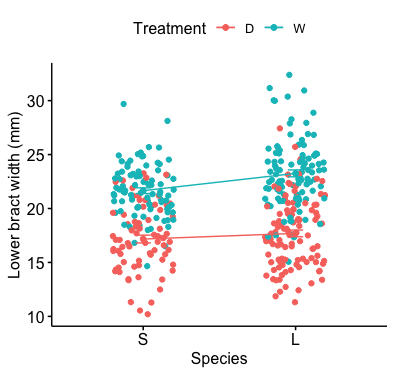
\includegraphics[width=70mm]{images/1_1.png}
\end{center}
  \caption{The mean plot with error bars for each treatment and species.}
  \label{fig1}
\end{figure}

A two-way ANOVA test was performed to analyze the effect of treatments and species on the LBW. Before perfoming the two-way ANOVA test, the assumption of two-way ANOVA is checked with diagnostic plots and test: Two-way ANOVA test assumes the data are normally distributed and variances across group are equal. The normality test for the LBW was done with Shapiro–Wilk test, and the test for homogeinity of the variances was done with Levene's test. There is no evidence to suggest that variances across group are statistically significantly different (F(3, 362) = 2.411, p = 0.067) as well as that the violation of normality (W = 0.99339, p = 0.1095). Thus two-way ANOVA test is conducted, the results is shown in Table \ref{tab1}.
\\
\begin{table}[h!]
\caption{\label{tab1}Two-way ANOVA results of the species and treatments on the LBW}
\begin{center}
\begin{tabularx}
{1\textwidth} { 
  >{\raggedright\arraybackslash}X 
  >{\centering\arraybackslash}X
  >{\centering\arraybackslash}X 
  >{\centering\arraybackslash}X 
  >{\centering\arraybackslash}X 
  >{\centering\arraybackslash}X 
  >{\raggedright\arraybackslash}X}
 \hline
& Df & Sum Sq & Mean Sq & F Value & Pr($>$F) \\ [0.5ex] 
 \hline
 sp & 1 & 52 & 52.0 & 5.740 & 0.0171 & * \\ 
 treat & 1 & 2363 & 2363.0 & 260.913 & $<$2e-16 & *** \\
 sp:treat & 1 & 26 & 26.1 & 2.886 & 0.0902 & . \\
 Residuals & 362 & 3279 & 9.1 \\
 \hline
 \multicolumn{7}{c}{Signif. codes:  0 ‘***’ 0.001 ‘**’ 0.01 ‘*’ 0.05 ‘.’ 0.1 ‘ ’ 1 }\\
 \hline
\end{tabularx}
\end{center}
\end{table}\\
The two-way ANOVA test revealed that there was not a statistically significant interaction between the effects of treatments and species (F(1, 362) = 2.886, p = 0.0902).
Simple main effects analysis showed that dry/wet treatment and species did have a statistically significant effect on LBW (p $<$ 0.0902, p = 0.0171 respectively). After the data were seen, post-hoc analysis - Tukey's HSD was performed to see if there was any pairs of treatment-species were different. Since the interaction did not have statistically significant effect, it was not included in Table \ref{tab2}
\begin{table}[h!]
\caption{\label{tab2}Tukey's HSD test on the two-way ANOVA results}
\begin{center}
\begin{tabularx}
{1\textwidth} { 
  >{\raggedright\arraybackslash}X 
  >{\centering\arraybackslash}X
  >{\centering\arraybackslash}X 
  >{\centering\arraybackslash}X 
  >{\centering\arraybackslash}X }
 \hline
 & diff & lwr & upr & p adj\\ 
 Species: S-L & -0.7597 & -1.3834 & -0.1361 & 0.0171 \\
 Treatment: W-D & 5.0732 & 4.4543 & 5.692 & 0 \\
 \hline\\ 
\end{tabularx}
\end{center}
\end{table}\\
\textbf{Conclusions}\\

The LBW of \textit{Dalechampia} that undergoes the wet treatment is 5.0723 mm wider than those with dry treatment, and the LBW of species L is 0.7597 mm wider than species S on average. There is no evidence showing the interaction between two factors, the dry/wet treatments and different species, on the width of lower bract of \textit{Dalechampia}.
\section{Effect of population density at birth on the mass of mountain goat with its sex as covariance}
\textbf{Background}\\

The density of living condition may affect on the growth of mountain goat. This research's purpose is to answer if the population density at birth (low/high) influence the mass of mountain goat, and if it was, controlling for sex, does the density still have an effect on the mass of goat? \\
\\
\textbf{Methods and Results}\\

A one-way ANOVA test was performed to compare the effect of population density on the mass of mountain goat. The one-way ANOVA test revealed in Table \ref{tab3} that there was a statistically significant difference in the mass of mountain goat between two density. (F(1, 4392) = 132.6, p = $<$2e-16).\\
\begin{table}[h!]
\caption{\label{tab3}One-way ANOVA results of the population density on the mass of mountain goat}
\begin{center}
\begin{tabularx}
{1\textwidth} { 
  >{\raggedright\arraybackslash}X 
  >{\centering\arraybackslash}X
  >{\centering\arraybackslash}X 
  >{\centering\arraybackslash}X 
  >{\centering\arraybackslash}X 
  >{\centering\arraybackslash}X 
  >{\raggedright\arraybackslash}X}
 \hline
& Df & Sum Sq & Mean Sq & F Value & Pr($>$F) \\ [0.5ex] 
 \hline
 density & 1 & 3736 & 3736 & 132.6 & $<$2e-16 & *** \\ 
 Residuals & 4392 & 123763 & 28 \\
 \hline
 \multicolumn{7}{c}{Signif. codes:  0 ‘***’ 0.001 ‘**’ 0.01 ‘*’ 0.05 ‘.’ 0.1 ‘ ’ 1 }\\
 \hline
\end{tabularx}
\end{center}
\end{table}\\

It is likely that the density does have a significant effect on the mass of goat, we continue to investigate for the difference in mass across low/high density when the variability is adjusted by including sex as covariance. To visualise the overall data, a mean plot of mass (Figure \ref{fig2} was constructed with errors bar for each sex, different colors indicate different density.\\
\begin{figure}[h!]
\begin{center}
  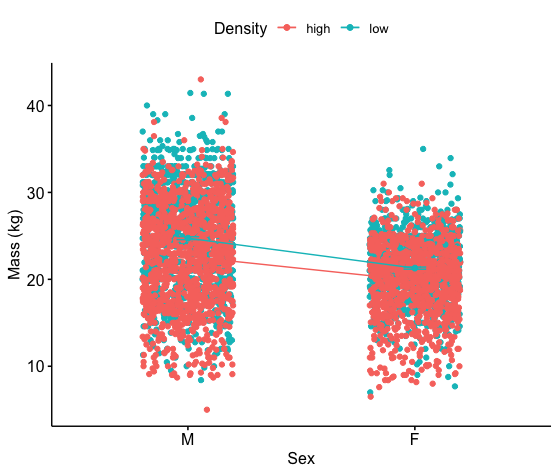
\includegraphics[width=70mm]{images/2_1.png}
\end{center}
  \caption{The mean plot with error bars for each sex and density.}
  \label{fig2}
\end{figure}\\

The ANCOVA test in Table \ref{tab4} revealed that there was sex and density did have a statistically significant effect on the mass of mountain goat (F(1, 4391) = 400.77, p = $<$2.2e-16; F(1,4391) = 137.49, p = $<$2.2e-16 respectively). To see how much the differences among group, post-hoc Tukey test was performed.
%ANCOVA table
\begin{table}[h!]
\caption{\label{tab4} ANCOVA results of the population density on the mass of mountain goat with sex as covariance}
\begin{center}
\begin{tabularx}
{1\textwidth} { 
  >{\raggedright\arraybackslash}X 
  >{\centering\arraybackslash}X
  >{\centering\arraybackslash}X  
  >{\centering\arraybackslash}X 
  >{\centering\arraybackslash}X 
  >{\raggedright\arraybackslash}X}
 \hline
& Sum Sq & Df & F Value & Pr($>$F) \\ [0.5ex] 
 \hline
 (Intercept) & 538991 & 1 & 29868.31 & $<$2.2e-16 & ***\\
 sex & 10351 & 1 & 400.77 & $<$2.2e-16 & *** \\ 
 density & 3551 & 1 & 137.49 & $<$2.2e-16 & *** \\
 Residuals & 113412 & 4391 \\
 \hline
 \multicolumn{6}{c}{Signif. codes:  0 ‘***’ 0.001 ‘**’ 0.01 ‘*’ 0.05 ‘.’ 0.1 ‘ ’ 1 }\\
 \hline
\end{tabularx}
\end{center}
\end{table}
%Tukey test table
\begin{table}[h!]
\caption{\label{tab5}Tukey test on the ANCOVA results}
\begin{center}
\begin{tabularx}
{1\textwidth} { 
  >{\raggedright\arraybackslash}X 
  >{\centering\arraybackslash}X
  >{\centering\arraybackslash}X 
  >{\centering\arraybackslash}X  
  >{\centering\arraybackslash}X }
 \hline
 & Estimate Std. & Error & t value & Pr($>$$|$t$|$)\\ 
 low-high & 1.7989 & 0.1534 & 11.73 & $<$2e-16 *** \\
 male-female & 3.0888 & 0.1543 & 20.02 & $<$2e-16 *** \\
\hline
\multicolumn{5}{c}{Signif. codes:  0 ‘***’ 0.001 ‘**’ 0.01 ‘*’ 0.05 ‘.’ 0.1 ‘ ’ 1 }\\
\hline\\
\end{tabularx}
\end{center}
\end{table}\\
\\
\textbf{Conclusions}\\

From Table \ref{tab5}, the mass of goat that live in a low density population is 1.79 $\pm$ 0.15 kg heavier than goat that live in high density population, and the male goat is 3.09 $\pm$ 0.15 kg heavier than female goat. With sex as covariance, the difference in mass of mountain goat born in different density is statistically significant.

\section{Appendix}
\textbf{R script for Part 1}
\begin{verbatim}
rm(list=ls())
install.packages(c("ggplot2","ggpubr","carData"))
library(ggplot2)
library(ggpubr)
library("car") 
# Set working directory
setwd("~/Documents/Study/MSc/BIOS13+14/14 exam")
# read data and remove NA in the data
dat = read.csv("exam2022_part1.csv")
dat<-dat[!is.na(dat$LBW),]

# The mean plot
ggline(dat,x='sp',y='LBW',color='treat',
       add = c("mean_se","jitter"), xlab = "Species", 
       ylab = "Lower bract width (mm)", legend.title="Treatment")

# Two-way ANOVA
twoANOVA = aov(LBW ~ sp*treat, data = dat)
summary(twoANOVA)

# Check the homogeneity of variance assumption
plot(twoANOVA,1)
leveneTest(LBW ~ sp*treat, data=dat)

# Check the normality assumption with Shapiro-Wilk test
plot(twoANOVA,2)
aov_residuals = residuals(object = twoANOVA)
shapiro.test(aov_residuals)

#Post-hoc tests
#TukeyHSD test
TukeyHSD(twoANOVA)



\end{verbatim}
\textbf{R script for Part 2}
\begin{verbatim}
rm(list=ls())
install.packages(c("ggplot2","ggpubr","carData","mvtnorm",
                   "survival","MASS","TH.data","multcomp"))
library(ggplot2)
library(ggpubr)
library(carData)
library(car)
library(mvtnorm)
library(survival)
library(MASS)
library(TH.data, warn.conflicts = FALSE)
library(multcomp)

# Set working directory
setwd("~/Documents/Study/MSc/BIOS13+14/14 exam")
# Read data and convert data to factor
dat = read.table("exam2022_part2.txt", header=T)
dat$density = as.factor(dat$density)
dat$sex = as.factor(dat$sex)

# Dependent variable: Mass
# Independent variable: Density 
# Covariate: Sex

# One-way ANOVA
one.way = aov(mass ~ density, data=dat)
summary(one.way)

# The mean plot
ggline(dat,x='sex',y="mass",color="density",
       add = c("mean_se","jitter"), xlab = "Sex", 
       ylab = "Mass (kg)", legend.title="Density")

# Fit ANCOVA model
ancova_model <- aov(mass ~ density + sex, data = dat)
Anova(ancova_model, type="III")

# post-Hoc test
postHocs_sex <- glht(ancova_model, linfct = mcp(sex = "Tukey"))
summary (postHocs_sex)
postHocs_density <- glht(ancova_model, linfct = mcp(density = "Tukey"))
summary(postHocs_density)
\end{verbatim}
\end{document}